% Options here are passed to the article class.
% Most common options: 10pt, 11pt, 12pt
\documentclass[10pt]{datasheet}

% Input encoding and typographical rules for English language
\usepackage[utf8]{inputenc}
\usepackage[english]{babel}
\usepackage[english]{isodate}

% tikz is used to draw images in this example, but you can
% also use \includegraphics{}.
\usepackage{graphicx}
\usepackage{float}
\usepackage{subcaption}

% These define global texts that are used in headers and titles.
\title{IM05: 1000 Non-Box Item RAM}
\author{Andrews54757}
\tags{item-memory, random-access, non-box}
\date{25 December 2024}
\revision{Revision 1}
\begin{document}
\maketitle

\section{Features}

\begin{itemize}
\item{Has 1000 different codes/item types. Items are stored in slots inside shulker boxes inside a dropper.}
\item{Random access. Can insert and retrieve items in constant time in any order.}
\item{Compact. 22x10x19 volume.}
\item{Maximum 55gt latency from call request to item.}
\end{itemize}

\section{Applications}
\begin{itemize}
\item{Dynamic code to item mapping.}
\item{Linked-list dynamic bulk mapping storage. See \href{https://www.youtube.com/watch?v=x6W-ZWkIdPE}{explanation video on Youtube}.}
\end{itemize}

\section{General Description}
The IM05 is able to store and retrieve non-box items with a specific decimal code. This may be useful for implementing dictionaries in an encoded dynamic sorting system. The device uses a 50-address item memory system with a hoppercart based slot cycling system to store and retrieve 1000 different items at near constant time.

\vfill\break

\begin{figure}[H]
    \centering
    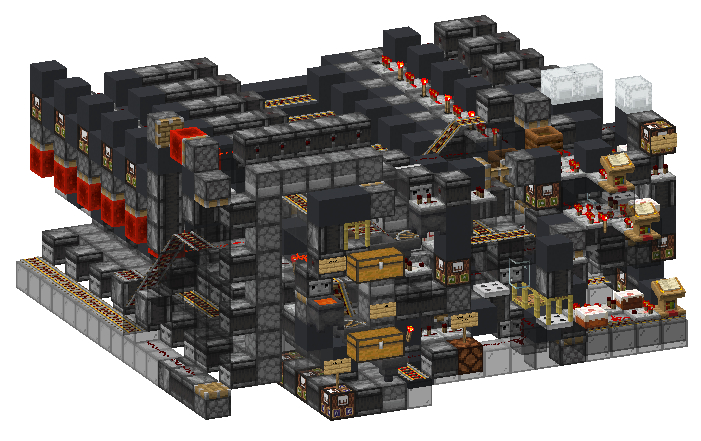
\includegraphics[width=0.48\textwidth]{image_1 (1).png}
    \caption{\centering 1000 Non-Box Item RAM}
\end{figure}

% For wide tables, a single column layout is better. It can be switched
% page-by-page.
\onecolumn

\section{Device Specifications}

\begin{table}[H]
    \caption{Inputs}
    \begin{tabularx}{\textwidth}{l | c | X}
        \thickhline
        \textbf{Name} & \textbf{Range} & \textbf{Description} \\
        \hline
        Code Digit 1 & 1-10 & First digit indicating row. \\
        Code Digit 2 & 1-10 & Second digit indicating column and slot. \\
        Code Digit 3 & 1-10 & Third digit indicating slot. \\
        \hline
        Execute swap & Pulse & Executes item swap with the given settings. \\
        \hline
        Item Input & Item & Item to be inserted/retrieved. \\
        \thickhline
\end{tabularx}
\end{table}

\begin{table}[H]
    \caption{Outputs}
    \begin{tabularx}{\textwidth}{l | c | X}
        \thickhline
        \textbf{Name} & \textbf{Range} & \textbf{Description} \\
        \hline
        Item Output & Item & Output for swap orders. \\
        \thickhline
\end{tabularx}
\end{table}

\begin{table}[H]
    \caption{Device Specifications}
    \begin{tabularx}{\textwidth}{l | c c c | c | X}
        \thickhline
        \textbf{Parameter} & \textbf{Min.} & \textbf{Typ.} & \textbf{Max.} &
        \textbf{Unit} & \textbf{Conditions} \\
        \hline
        Latency & 36 & - & 55 & gt & From call request to item. \\
        \hline
        Hopper Count & & 88 & & Hoppers & \\
        \hline
        MC Version & 1.17 & 1.19.3 & - & MCV & Latest version at time of writing: 1.21.4\\
        \hline
        Dimensions & & 22 x 10 x 19 & & Blocks & \\
        \thickhline
\end{tabularx}
\end{table}

\section{Testing Data}

\begin{table}[H]
\caption{Executed Tests}
\begin{tabularx}{\textwidth}{l | X}
    \thickhline
    \textbf{Test} & \textbf{Result} \\
    \hline
    Insertion & Items were successfully inserted in all positions. \\
    \hline
    Retrieval & Items were successfully retrieved from all positions. \\
    \thickhline
\end{tabularx}
\end{table}
    
\section{Download Information}
\begin{table}[H]
    \caption{Download Information}
    \begin{tabularx}{\textwidth}{l | l | l | X}
        \thickhline
        \textbf{Identifier} & \textbf{MC} & \textbf{File} & \textbf{Description} \\
        \hline
        IM05 & 1.19.3 & \href{https://github.com/Soontech-Annals/Archive/blob/8413f90a054b6c415703bae02badeba7541344f6/Archive/item-memory/IM05\%201000\%20Non-Box\%20Item\%20RAM/IM05\_1000\_Non-Box\_Item\_RAM.litematic?raw=1}{IM05\_1000\_Non-Box\_Item\_RAM.litematic} & Schematic of device. Includes dummy item storage. \\
        \hline
        \thickhline
    \end{tabularx}
\end{table}

\end{document}

